
\chapter{Conceitos iniciais}
\label{chap:conceitos_iniciais}

	\section{Exploit/Vulnerabilidade}
	O primeiro termo que devemos definir neste trabalho é exploit. Mas antes dele,
	trataremos de vulnerabilidade - pois eles têm uma ligação estreita.
	Podemos definir vulnerabilidade como uma falha em um sistema que permite
	a um atacante usá-lo de uma forma não prevista pelo projetista \cite{Anley2007}.
	Ou seja, uma vulnerabilidade implica a possibilidade de uso indevido de um sistema.
	Os passos necessários para explorar essa fraqueza, ou mesmo o código (programa) que pode tirar
	proveito da vulnerabilidade é descrito como exploit.
	Um exploit surge apenas quando há uma vulnerabilidade - mas podem existir
	vulnerabilidades para as quais não exista exploit.


	\section{Conceitos básicos}
	Neste trabalho iremos tratar de exploits na arquitetura x86 de 32 bits. Trata-se da arquitetura de computadores
	pessoais mais difundida nos dias de hoje. Mas boa parte do estudo realizado pode ser aplicada
	a praticamente qualquer outra arquitetura.

	\section{Gerência de memória}
	O controle da memória é um ponto crítico. Falhas nele acabam resultando em vulnerabilidades 
	gravíssimas. Faremos uma breve abordagem sobre o gerenciamento de memória sobre
	o ponto de vista dos exploits.

	Um primeiro ponto a destacar sobre a memória é um princípio básico que norteia
	quase todas as arquiteturas modernas. Dados e instruções não são diferenciados na memória.
	Ou seja, não há uma separação rígida entre instruções que compõem um programa e os dados
	sobre os quais opera. Essa característica foi herdada da arquitetura básica de von Neumann.
	Como veremos a seguir, essa decisão de design, com origem nos anos 1940, embora tenha
	facilitado a evolução dos computadores, abriu caminhos para os exploits que conhecemos hoje. 

	Abaixo descrevemos o layout básico da memória de um processo em um sistema UNIX.
	Ele pode ser separado em 6 partes fundamentais:
	\begin{description}
		\item[text]
			A parte que contém as instruções do programa - seu código propriamente dito.
			Seu tamanho é fixo durante a execução e ela não deve possibilitar escrita.
		\item[data]
			Contém variáveis globais já inicializadas. Seu tamanho é fixo durante a execução.
		\item[bss]
			Nome de origem história significando Block Started by Symbol. Área da memória responsável
			por armazenar variáveis globais	não inicializadas. Como text e data, bss também tem tamanho 
			fixo conhecido desde o início do processo. 
		\item[Heap]
			Espaço para variáveis alocadas dinamicamente. A chamada de sistema sbrk é responsável
			pelo controle do crescimento/encolhimento desse espaço. Bibliotecas geralmente facilitam a vida
			do programador disponibilizando interfaces mais amigáveis como malloc() e free(). Assim a biblioteca
			se encarrega de chamar sbrk() para diminuir/aumentar o Heap. Ela cresce do endereço mais baixo para o
			mais alto.
		\item[Stack]
			Mantém controle das chamadas de funções. Possibilita a recursividade. Logo, possui
			tamanho variável - crescendo do endereço mais alto para o mais baixo (sendo antagonista do Heap - ver
			figura \ref{fig:regioes_memoria}). 
			Esse crescimento é que torna possível que uma chamada de função que tenha seus dados
			sobrescritos influencie numa chamada de função anterior. Esse é o princípio do buffer overflow - tratado
			posteriormente.
		\item[Enviroment]
			A última porção de memória do processo guarda uma cópia das variáveis de ambiente do sistema.
			Essa seção possui permissão de escrita, mas como bss, data e text, possui tamanho fixo.
	\end{description}

	\begin{figure}
		\begin{center}
		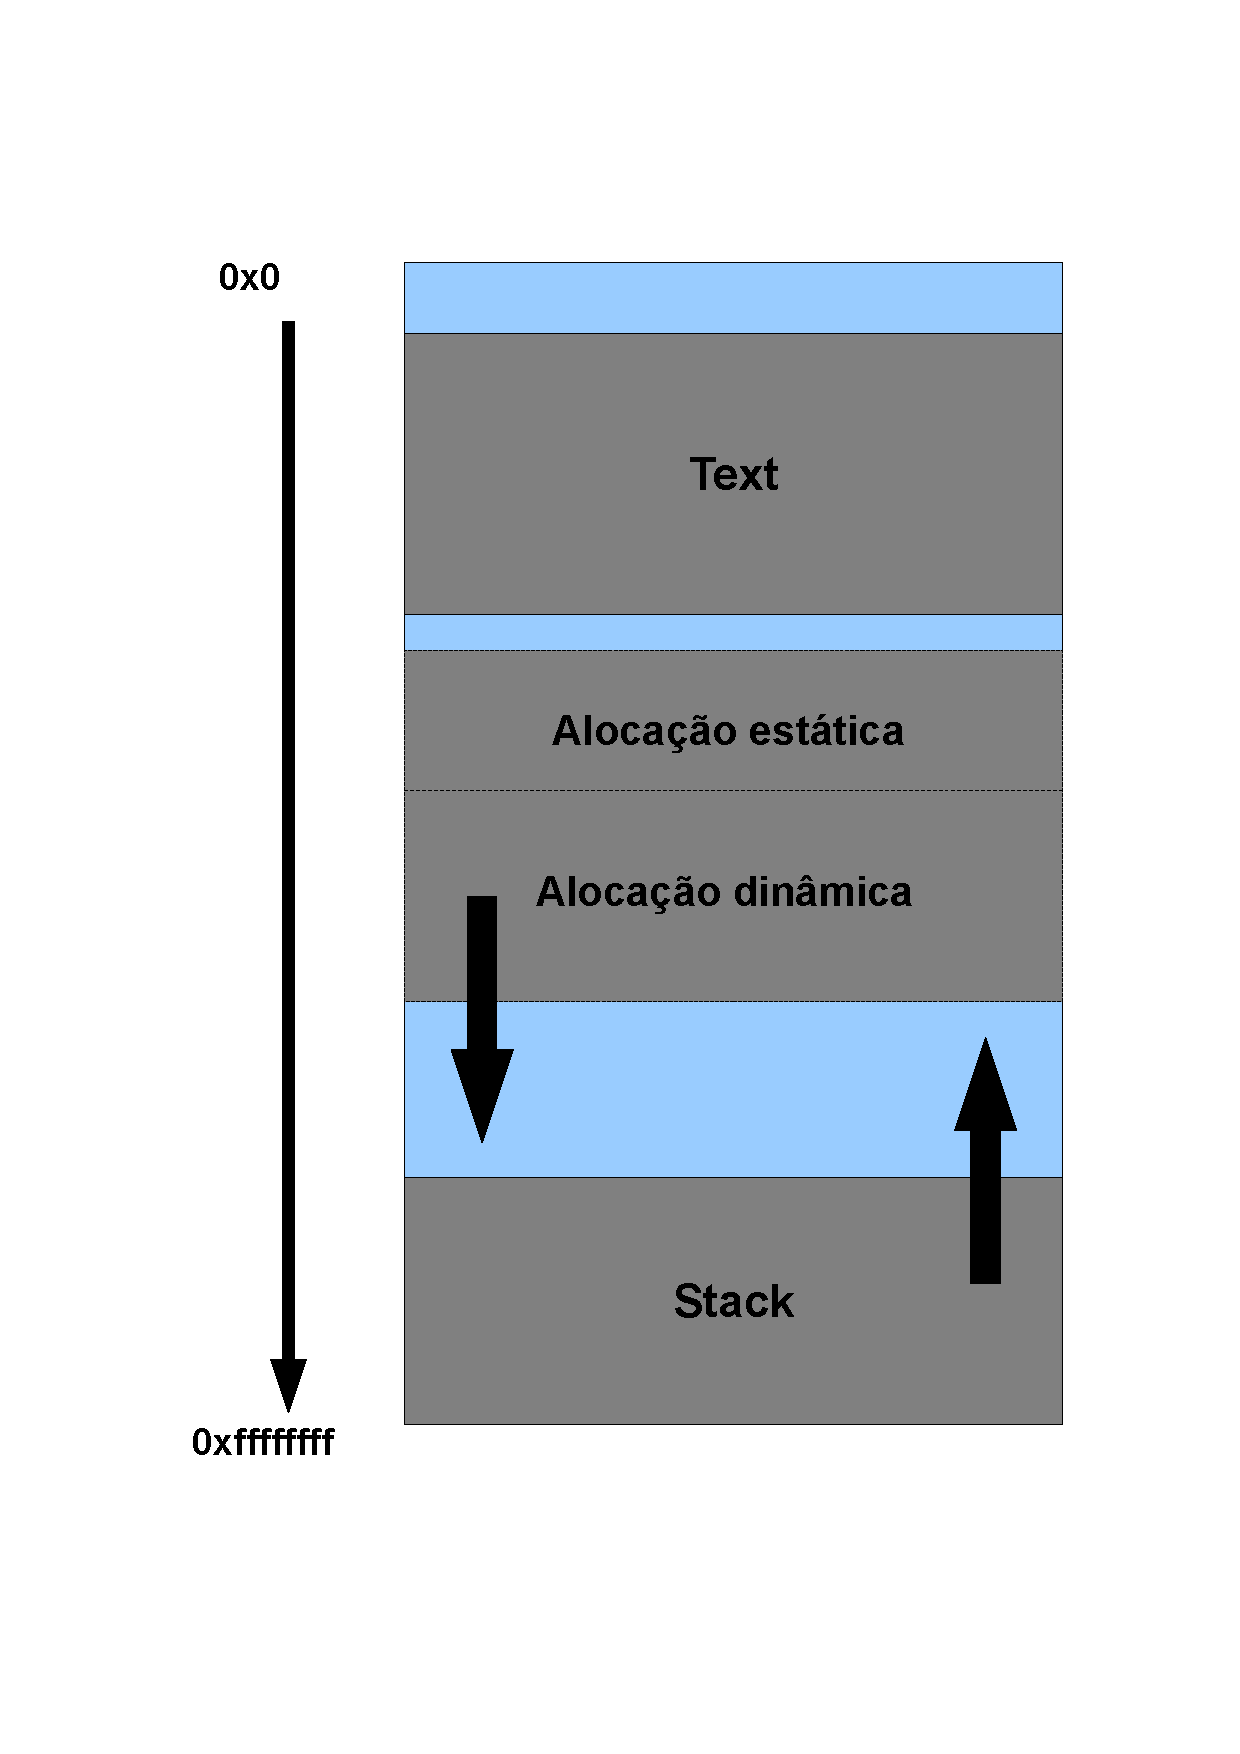
\includegraphics[width=0.45\textwidth]{regioes_memoria.pdf}
		\caption{Regiões de memória em um processo.}
		\label{fig:regioes_memoria}
		\end{center}
	\end{figure}

	\section{Funcionamento mais detalhado do Stack}

	\section{Funcionamento mais detalhado do Heap}
	A porção de memória correspondente ao heap possibilita ao programador alocar dinamicamente memória
	que fica disponível durante toda a execução para qualquer chamada de função. Diferentemente
	da memória alocada no stack - que é perdida quando a função retorna.

	\section{Registradores de controle}
	Uma parte fundamental da arquitetura que deve ser mencionada são os registradores que possuem
	relação direta com o gerenciamento da memória.
	Talvez o mais importante (na arquitetura base do estudo IA32) seja o EIP(Extended Instruction Pointer).
	Ele indica o endereço da próxima instrução. Sobrescrevê-lo equivale obter o controle
	do fluxo de um processo.
	Além dele, destacamos EBP(Extended Base Pointer) e ESP(Extended Stack Pointer).
	ESP indica o endereço do último valor inserido na pilha.
	O EBP indica o início da pilha para aquela chamada de função. É usado para referenciar variáveis
	locais da função.


